\documentclass[a4paper]{sbgames}               % final
%\usepackage[scaled=.92]{helvet}
\usepackage{times}
\usepackage{graphicx}

%% use this for zero \parindent and non-zero \parskip, intelligently.
\usepackage{parskip}

%% the 'caption' package provides a nicer-looking replacement
\usepackage[labelfont=bf,textfont=it]{caption}

\usepackage{url}
\usepackage[]{algorithm2e}
\usepackage{array}
\newcolumntype{L}{>{\centering\arraybackslash}m{3cm}}

%% Paper title.
\title{Developing an Accessible One-Switch Game for Motor Impaired Players}


%% Author and Affiliation (multiple authors). Use: and between authors

\author{Fernando L. Souza: Lucas C. Medeiros: Marcos F. Parreiras}

%\affiliation{Departamento de Computa\c{c}\~{a}o \\
%        Centro Federal de Educa\c{c}\~{a}o Tecnol\'{o}gica de Minas Gerais \\
%        Belo Horizonte, Brasil
%}

\affiliation{ Centro Federal de Educa\c{c}\~{a}o Tecnol\'{o}gica de Minas Gerais, Departamento de Computa\c{c}\~{a}o, Brasil
}

\contactinfo{nandolcs@hotmail.com \\
             *cmedeiros.lucas@gmail.com \\
             *marcosfparreiras@gmail.com
}
%\contactinfo{author1@email.com \\
%             author2@email.com
%}
%% Keywords that describe your work.
\keywords{accessibility. motor impairments. digital game. one switch.}

%% Start of the paper
% Attention: As you need to insert EPS images in Postscript, 
% you need to insert PDF images into PDFs. 
% In the text, extensions cancbe omitted (latex use .eps, pdflatex get .pdf) 
% To convert them: epstopdf myimage.eps
\begin{document}

%\teaser{
 % 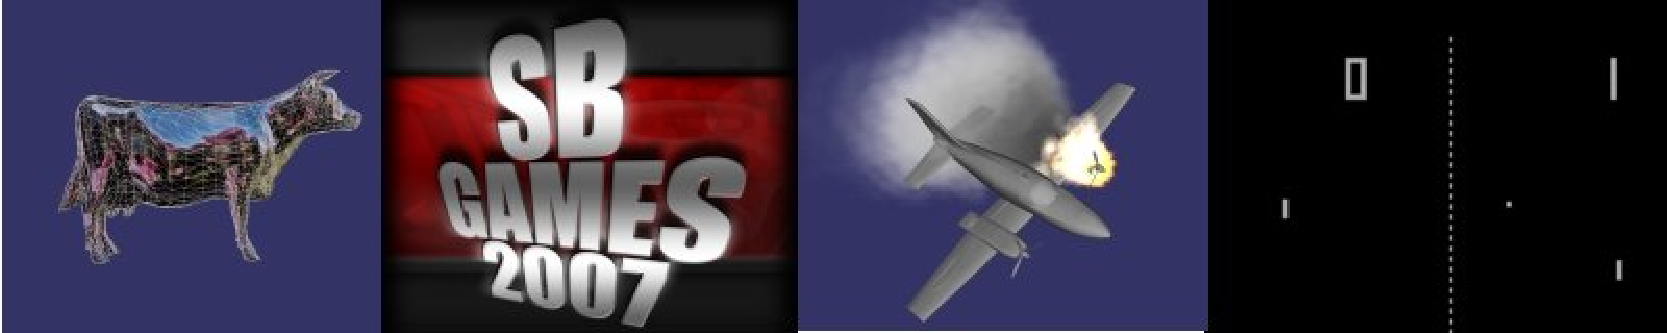
\includegraphics[width=\linewidth]{sample.pdf}
  %\caption{Optional image}
%}

%% The ``\maketitle'' command must be the first command after the
%% ``\begin{document}'' command. It prepares and prints the title block.

\maketitle

%% Abstract section.

\begin{abstract}

O Resumo vai aqui
\end{abstract}

%% The ``\keywordlist'' command prints out the keywords.
\keywordlist
\contactlist

\section{Introdução}
\label{sec:introducao}

Introdução

Com a chegada da plataforma mobile, a possibilidade de se alcançar grande sucesso com software aumentou significativamente. No caso dos aplicativos desenvolvidos para esta plataforma, o software está sempre ao alcance do usuário final, permitindo que seja utilizado a partir de um simples toque.

O mercado de jogos é um dos que tem se aproveitado desta versatilidade e, com isso, vários são os casos de jogos que vêm ganhando grande popularidade e alcançando a casa dos milhões de downloads, como é o cado, por exemplo, dos jogos \textit{Candy Crush Saga} e \textit{Clash of Clans}. Um caso bastante especial de jogo a se destacar em meio a este mercado tão concorrido foi o \textit{Flappy Bird}: um dos jogos mais emblemáticos e icônicos desde o início deste novo mercado mobile. Possuindo uma estrutura extremamente simples, este jogo teve uma ascensão meteórica, alcançando o topo das principais lojas de aplicativos, \textit{Google Play} e \textit{App Store}, e chegando a arrecadar cerca de cinquenta mil dólares por dia a partir de anúncios no aplicativo \cite{Warren2014}. Após tamanho sucesso, seu fim foi tão repentino quanto seu surgimento, como é relatado na próxima seção.






\section{Uma Breve História do Jogo}
\label{sec:historia}


\section{Componentes}
\label{sec:componentes}


\section{Fórmula do Sucesso}
\label{sec:sucesso}


\subsection{Conclusão}
\label{sec:conclusao}



\bibliographystyle{sbgames}
\bibliography{template}
\end{document}
